\chapter{Chromium Dimer Simulation with Fast SHCI}
In this chapter, I apply the fast SHCI method to the chromium dimer system.
I first perform an accurate calculation at the equilibrium geometry, and then perform a slightly less accurate calculation for several squeezed or stretched geometries and obtain the entire potential energy surface.

\section{Introduction}

Chromium dimer is a challenging strongly-correlated system
that has been used as a benchmark molecule for a variety of methods~\cite{Scu-JCP-91,KurYan-JCP-11,PurZhaKra-JCP-15,MaManOlsGag-JCTC-16,VanMalVer-JCTC-16,GuoWatHuSunCha-JCTC-16}.
In this chapter, we use the fast heat-bath configuration interaction method to calculate both the energy at the equilibrium geometry and entire potential energy curve.

For the equilibrium geometry, we include in our variational wavefunction two billion most important determinants, which are two orders of magnitudes more than ever done in other selected-CI based methods.
This allows us to achieve significantly higher accuracy, which even beats the accuracy of well-developed methods, such as the density matrix renormalization group (DMRG).
Section~\ref{sec:eq} presents the results.

%For the entire potential energy curve calculation, we include in our Hilbert space up to 28 active electrons with a cc-pVDZ basis.
For the entire potential energy curve calculation, we correlate up to 28 electrons in a cc-pVDZ basis.
The resulting Hilbert space of $5 \times 10^{29}$ determinants is several orders of magnitude larger than that used in other
systematically improvable methods.
Our results match well with the experiments at and near the equilibrium geometry.
Section~\ref{sec:curve} presents the results.

\section{Equilibrium Geometry}
\label{sec:eq}
In this section\footnote{This section was published in Ref.~\cite{li2018fast}}, we examine the chromium dimer at the equilibrium bond length of 1.68 $\AA$. % angstroms.
%We use a cc-pVDZ basis with active semi-core electrons.

We use a relativistic exact two-component (X2C) Hamiltonian, the cc-pVDZ-DK basis, and we correlate the valence and the semi-core electrons.
This gives an active space of (28e, 76o) and a Hilbert space of $5\times10^{29}$ determinants, which is far beyond the reach of FCI.
We show how we obtain an accurate estimate of the FCI energy in this large active space with our improved SHCI algorithm.

We use PySCF~\cite{SunCha_etal_PySCF-ComMolSci-18} to generate the molecular orbital integrals for orbitals that minimize the HCI variational
energy for $\epsilon_1=2\times 10^{-4}$~Ha, using the method of Ref.~\cite{SmiMusHolSha-JCTC-17}.
We perform SHCI with several $\epsilon_1$ values from $5\times10^{-5}$ to $3\times10^{-6}$~Ha.
The Hamiltonian matrix is constructed only once.
% The Hamiltonian matrix is stored in memory and so needs to be constructed only once.
%We keep the ratio between $\epsilon_2$ and $\epsilon_1$ to $10^{-6}$ and the target error for the stochastic perturbation to 0.01 mHa.
We use very small values of $\epsilon_2 = 10^{-6} \epsilon_1$  to ensure that the perturbative correction is exceedingly well converged,
and choose the target error for the stochastic perturbation energy to be $10^{-5}$~Ha.

%The improved SHCI is fast enough that we can use over two billion variational determinants and include at least trillions of effective perturbative determinants.
The improved SHCI is fast enough that we can use over two billion variational determinants, and stochastically include the contributions of at least trillions of perturbative determinants.
The largest variational calculation, where we iteratively find and diagonalize 2 billion determinants
for $\epsilon_1=3.0\times10^{-6}$~Ha, takes only one day on 8 nodes, each of which has 4 Intel Xeon E7-8870 v4 CPUs.
The corresponding perturbative calculation takes only 6 hours using only one of these nodes. 
During that perturbative calculation, we skip the deterministic step, perform a pseudo-stochastic step with $\epsilon_2^{\rm psto}=1\times10^{-7}$~Ha, and a stochastic step with $\epsilon_2=3\times10^{-12}$~Ha.
{\color{black}
We skip the deterministic step here because $\epsilon_1=3 \times 10^{-6}$ is already close to our
default $\epsilon_2^{\rm dtm}$ of $2 \times 10^{-6}$ so skipping this won't affect the efficiency
of subsequent steps much.
}
The pseudo-stochastic step uses 25 batches, each of which has about 8.9 billion determinants.
We evaluate only one of them, from which we obtain an estimate of the total correction for all the 25 batches (223 billion determinants) to be -0.011681(1)~Ha.
Since the estimated error is already much smaller than our target error, we skip the remaining 24 batches.
The pseudo-stochastic step takes 1.6 hours.
The stochastic step uses 128 batches and 6 million variational determinants in each sample,
which results in about 3.7 billion determinants per batch.
We use 10 samples and obtain the additional correction from $\epsilon_2=3.0\times10^{-12}$~Ha to be -0.001203(6)~Ha.
The combined uncertainty of the entire semistochastic perturbation stage is 6~$\mu$Ha.
It is hard to estimate how many determinants are stochastically included for $\epsilon_2=3\times10^{-12}$~Ha,
so we estimate a lower bound with $\epsilon_2^{\rm psto}=1.4\times10^{-8}$~Ha and obtain 1.8 trillion unique perturbative determinants.
Hence, with $\epsilon_2=3\times10^{-12}$~Ha (the value we are actually using) we stochastically estimate contributions from
at least trillions of unique perturbative determinants and obtain better than $10^{-5}$~Ha statistical uncertainty in 6 hours using only one node.
%why?
%This brings the accuracy selected-CI to a whole new level and enables us to obtain an estimation of the FCI energy with sub-millihartree uncertainty in this large active space.

These large calculations enable us to obtain an estimate of the FCI energy with sub-millihartree uncertainty in this large active space.
Table~\ref{tab:Cr2} reports the results.


\begin{table}
  \begin{center}
  \begin{tabular}{| c | c | c | c |}
  \hline
  $\epsilon_{1}$ (Ha) & $N_\V$ & $E_{\rm var}$ (Ha) & $E_{\rm total}$ (Ha) \\
  \hline\hline
  $5.0\times10^{-5}$ & 24M & -2099.863816 & -2099.909741(7) \\
  \hline
  $3.0\times10^{-5}$ & 53M & -2099.875327 & -2099.912356(7) \\
  \hline
  $2.0\times10^{-5}$ & 102M & -2099.883027 & -2099.914132(8) \\
  \hline
  $1.0\times10^{-5}$ & 309M & -2099.893761 & -2099.916595(1) \\
  \hline
  $7.0\times10^{-6}$ & 539M & -2099.898165 & -2099.917540(1) \\
  \hline
  $5.0\times10^{-6}$ & 911M & -2099.901781 & -2099.918306(3) \\
  \hline
  $3.0\times10^{-6}$ & 2.00B & -2099.906322 & -2099.919205(6) \\
  \hline
  0.0 (Extrap.) & - & \multicolumn{2}{ c |}{-2099.9224(6)} \\
  \hline
  \end{tabular}
  \end{center}
  \caption{Results for Cr$_2$ at r=1.68\AA\ in the cc-pVDZ-DK basis.
  The active space is (28e, 76o).
  $N_\V$ is the number of variational determinants.
  $\epsilon_2 = 10^{-6} \epsilon_1$.
  We use weighted quadratic extrapolation, shown in Fig.~\ref{fig:extrapolation}, to obtain the FCI limit
  corresponding to $\Delta E=0$.}
  \label{tab:Cr2}
\end{table}

\begin{figure}
  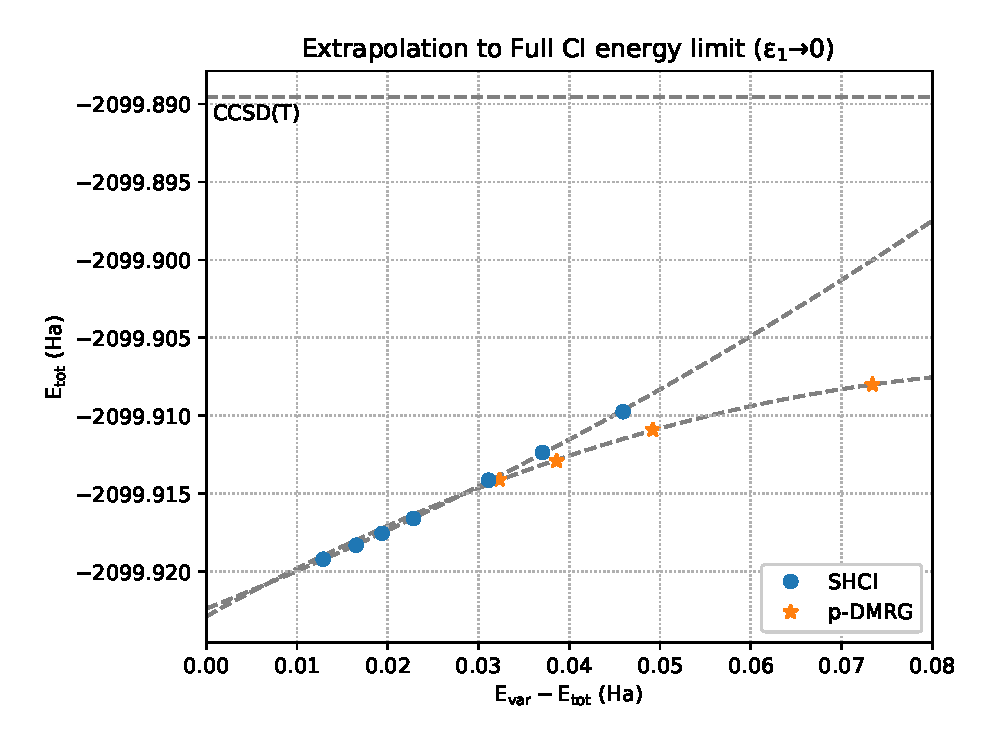
\includegraphics[width=\linewidth]{figs/extrapolate.eps}
  \caption{Weighted quadratic extrapolation of the Cr$_2$ ground state energy.
  The weight of each point is $(E_{\rm var} - E_{\rm tot})^{-2}$.
  The extrapolated energy is $-2099.9224(6)$, where the uncertainty comes from the difference between linear extrapolation and quadratic extrapolation.
  The p-DMRG extrapolation and the CCSD(T) value are also shown.
}
%   {\color{red} I don't remember -- where did this CCSD(T) value come from?  Does it matter if it is CCSD(T) or UCCSD(T)?}
  \label{fig:extrapolation}
\end{figure}

We extrapolate our results using a weighted quadratic fit
and obtain for the ground state energy, $-2099.9224$~Ha as $\Delta E\to0$.
The weight of each point is $(E_{\rm var} - E_{\rm tot})^{-2}$.
Fig.~\ref{fig:extrapolation} shows the computed energies and the extrapolation.
We also perform a weighted linear fit and use the difference of the extrapolated values from the quadratic and the linear fits (0.6~mHa) as the uncertainty.
%If we look at the trends of the data points in Fig.~\ref{fig:extrapolation}, we can see that 0.55~mHa is a reasonable estimation of the uncertainty.
%In summary, the estimated FCI energy of Cr$_2$ in the cc-pVDZ basis with active semi-core electrons is $-2099.9224(6)$~Ha.
In summary, the estimated FCI energy of Cr$_2$ in the cc-pVDZ-DK basis with 28 correlated electrons and the relativistic X2C Hamiltonian
%(the rest of the electrons are frozen in
%Hartree-Fock orbitals)
is $-2099.9224(6)$~Ha.

\begin{figure}
  \begin{center}
  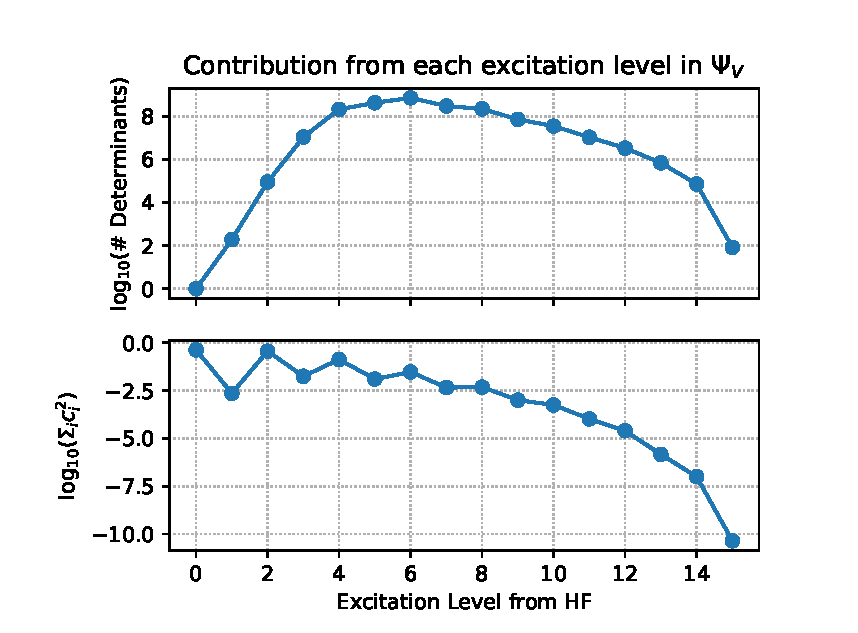
\includegraphics[width=0.9\linewidth]{figs/excitation.eps}
  \caption{Contribution from each excitation level to the variational wavefunction for Cr$_2$ with $2 \times 10^9$ determinants.
  Determinants with up to 15 excitations are present in the variational wavefunction.
%  {\color{red} Leave out the top plot, since sums of squared magnitudes is meaningful, but number of nonzero magnitudes is a meaningless quantity? Well, it does mean that there were several higher-order excitations that are more important than lower-order ones.}
}
  \label{fig:excit}
  \end{center}
\end{figure}

We compare our result with DMRG and p-DMRG, which are the only essentially exact methods that have been applied to this large active space of the chromium dimer.
The DMRG calculations use up to bond dimension $M=16000$ and obtain an extrapolated energy of $-2099.9195(27)$~Ha (default schedule) and $-2099.9192(24)$ (reverse schedule)~\cite{GuoLiCha-JCTC-18}.
%These two values are similar to our most accurate data point but higher than our extrapolated result by 3~mH, which is about one standard error of the DMRG results.
These two values are similar to our most accurate data point but higher than our extrapolated result by 3~mH, which is about the estimated error of the DMRG results.
%The p-DMRG calculations use up to $M=4000$ and obtain an extrapolated energy of $-2099.9201$~Ha~\cite{GuoLiCha-JCTC-18}.
The p-DMRG calculations use up to $M=4000$ and extrapolated energy obtained from a linear fit is $-2099.9201$~Ha~\cite{GuoLiCha-JCTC-18}.
If instead, we perform a weighted quadratic fit (shown in Fig.~\ref{fig:extrapolation}), the extrapolated energy is $-2099.9225$~Ha,
in perhaps fortuitously good agreement with our result of $-2099.9224(6)$~Ha.  However, the extrapolation uncertainty is larger than the SHCI extrapolation uncertainty.
In contrast, the CCSD(T) energy is considerably higher.
%In summary, our extrapolated value agrees with DMRG's and p-DMRG's extrapolated results but we achieve a smaller uncertainty.

%One of the merits of selected-CI is the ability to take higher-order excitations into account accurately.
%One of the merits of selected-CI methods is the ability to include higher-order excitations.
One of the merits of selected-CI methods is the ability to include all excitations, regardless of excitation level.
To see the contribution from each excitation level we plot the number of selected determinants and the $\sum_i \left|c_i\right|^2$ versus excitation level in Fig.~\ref{fig:excit}.
Determinants with excitation levels up to 15 excitations are present in the variational wavefunction even though we are using optimized orbitals.
(Using Hartree-Fock orbitals, we expect that determinants with even higher excitation levels will be present.)
%This implies that truncating the CI or the CC at the double or the triple excitation level may not give reliable results for such strongly correlated systems.
This implies that truncating the CI expansion at the double, triple or quadruple excitation levels (which is the most that is usually done in systematic
CI expansions), will give poor energies for such strongly correlated systems.

\section{Potential Energy Surface}
In addition to the energy at equilibrium geometry, I also obtain the entire potential energy curve of the chromium dimer.

We calculate the potential energy curves, first correlating just the 12 valence (3d, 4s) electrons, and then correlating
also the semi-core (3s,
3p) electrons, making a total of 28 correlated electrons.
For 12 correlated electrons, we study the basis set dependence by calculating the curves for cc-pVDZ, cc-pVTZ, and cc-pVQZ basis sets.
%We examine the effect of correlating the semi-core electrons, i.e., we
%We exam the results from using the cc-pVDZ-DK basis and the cc-pVTZ-DK basis, and also the effects of correlating only the 12 valence electrons and correlating 28 electrons from both the valence and the semi-core.
The largest active space in our calculations is (28e, 76o), which gives a Hilbert space of $5\times10^{29}$ determinants, far beyond the reach of FCI.
%Due to the high efficiency of our algorithm, we can calculate each data point on this curve with such huge active space and obtain the entire potential energy curve.

We use both PySCF~\cite{SunCha_etal_PySCF-ComMolSci-18} and our program to generate the molecular orbital integrals for orbitals that minimize the HCI variational
energy for $\epsilon_1=2\times 10^{-4}$~Ha, using an improved version of the method of Ref.~\cite{SmiMusHolSha-JCTC-17}.
For 12 correlated electrons, we use CAS-core orbitals, and for 28 correlated electrons, we use the HF-core orbitals.
For the former, the potential energy curves obtained from HF-core and CAS-core orbitals differ greatly,
whereas for the latter, there is essentially no difference between HF-core and CAS-core curves.
We perform SHCI with several $\epsilon_1$ values from $2\times10^{-4}$ to $5\times10^{-6}$~Ha.
%The Hamiltonian matrix is constructed only once for each geometry and each active space.
The sparse Hamiltonian matrix is stored in memory and so needs to be constructed only once for each geometry and each active space.
%We keep the ratio between $\epsilon_2$ and $\epsilon_1$ to $10^{-6}$ and the target error for the stochastic perturbation to 0.01 mHa.
For the perturbative correction calculation, we set $\epsilon_2 = 0$  to include the entire Hilbert space.

%The improved SHCI is fast enough that we can use over two billion variational determinants and include at least trillions of effective perturbative determinants.
The improved SHCI is fast enough that we can use more than one billion variational determinants and stochastically include the corrections from at least trillions of perturbative determinants for each geometry.

We extrapolate the energies for each geometry with a weighted quadratic fit
and obtain for the ground state energy as $\Delta E\to0$.
The weight of each point is $(E_{\rm var} - E_{\rm tot})^{-2}$.
Then we interpolate the points for each active space with cubic spline interpolation.
Fig.~\ref{fig:cr2raw} presents the most accurate raw data points and the extrapolated curve for the 28 correlated electrons case.

\label{sec:curve}
\begin{figure}
  \begin{center}
  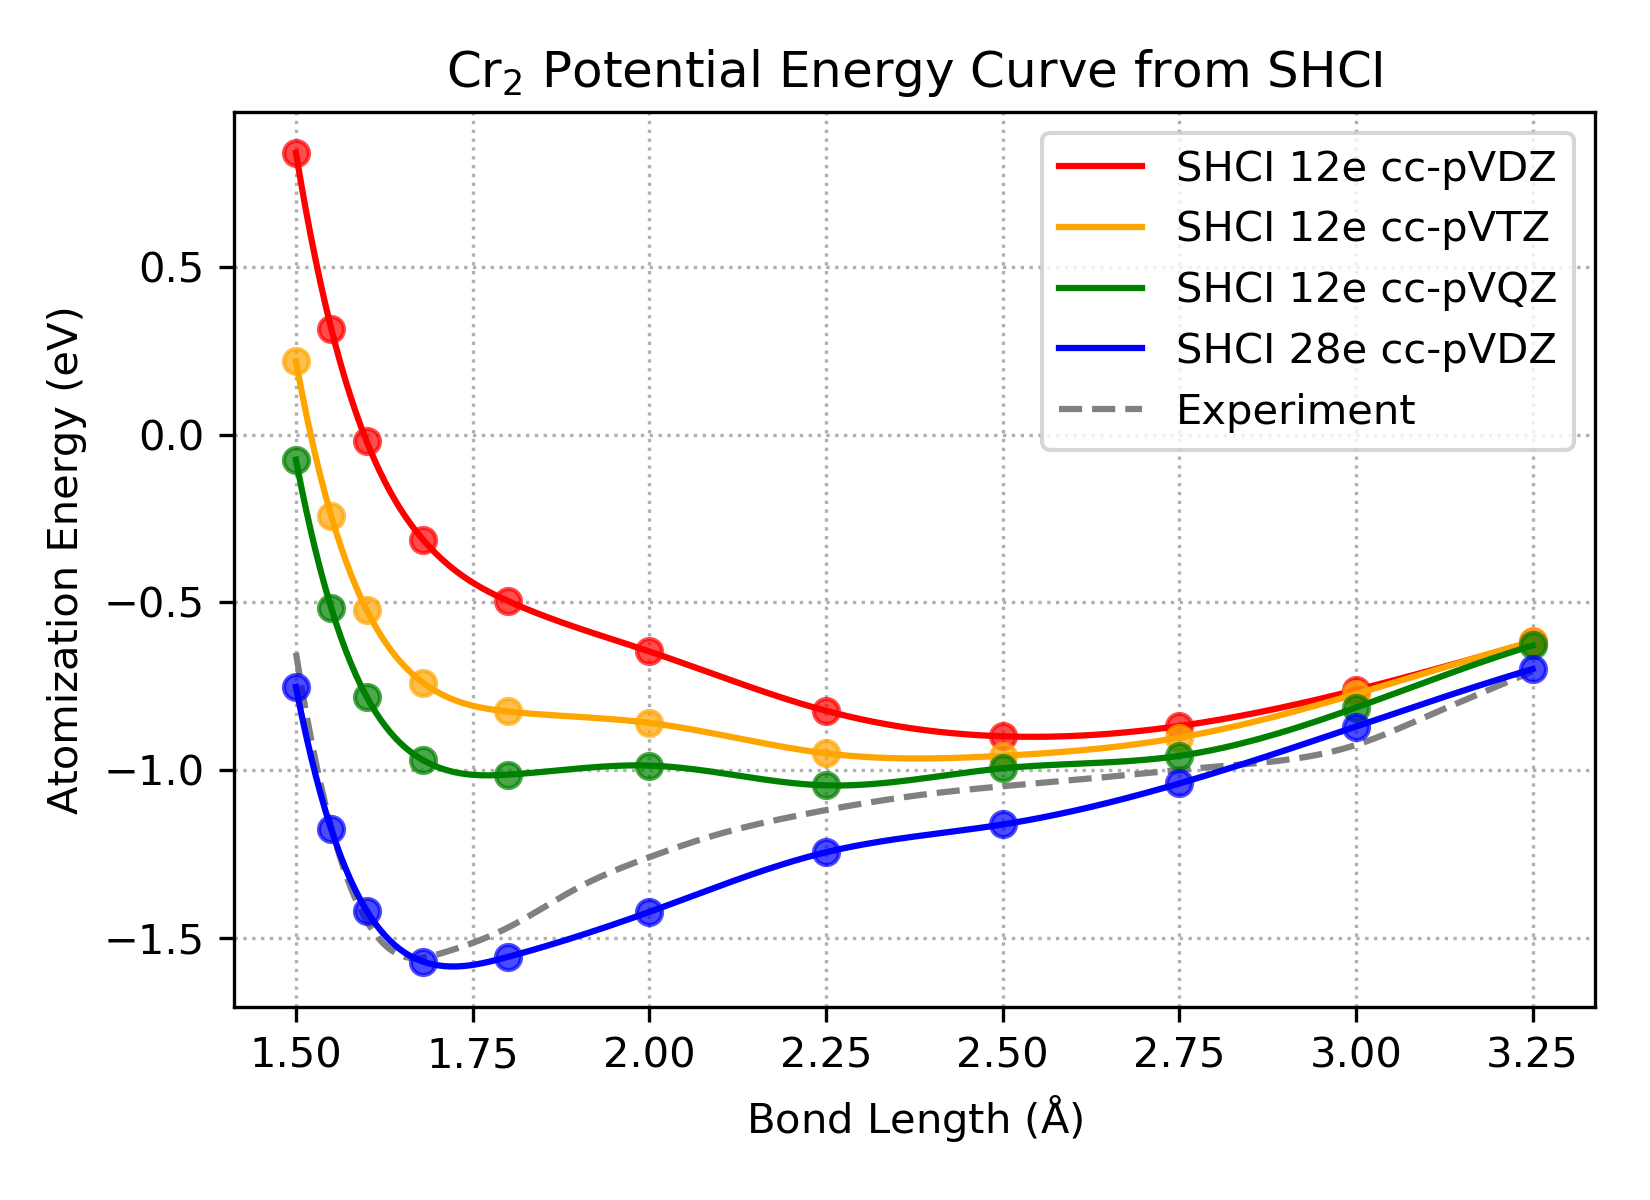
\includegraphics[width=0.9\linewidth]{figs/cr2curve.png}
  \caption{Comparison of SHCI potential energy curves of Cr$_2$, correlating 12 or 28 electrons, with experiment.
  The shape of the experimental data is deduced from measuring 29 vibrational states using negative-ion photoelectron spectroscopy~\cite{casey1993negative}.
  %We can see that using only 12 active electrons from the shell cannot produce a good agreement to the experimental data.
  %By including 10 additional electrons from the semi-core into the active space, the agreement with experimental data is much better.
  The potential energy curves from the 12-correlated-electron calculations agree poorly with experiment, though the agreement
  improves upon increasing the basis size.
  The 28-correlated-electron calculation agrees much better with experiment.
  }
  \label{fig:cr2curve}
  \end{center}
\end{figure}

\begin{figure}
  \begin{center}
  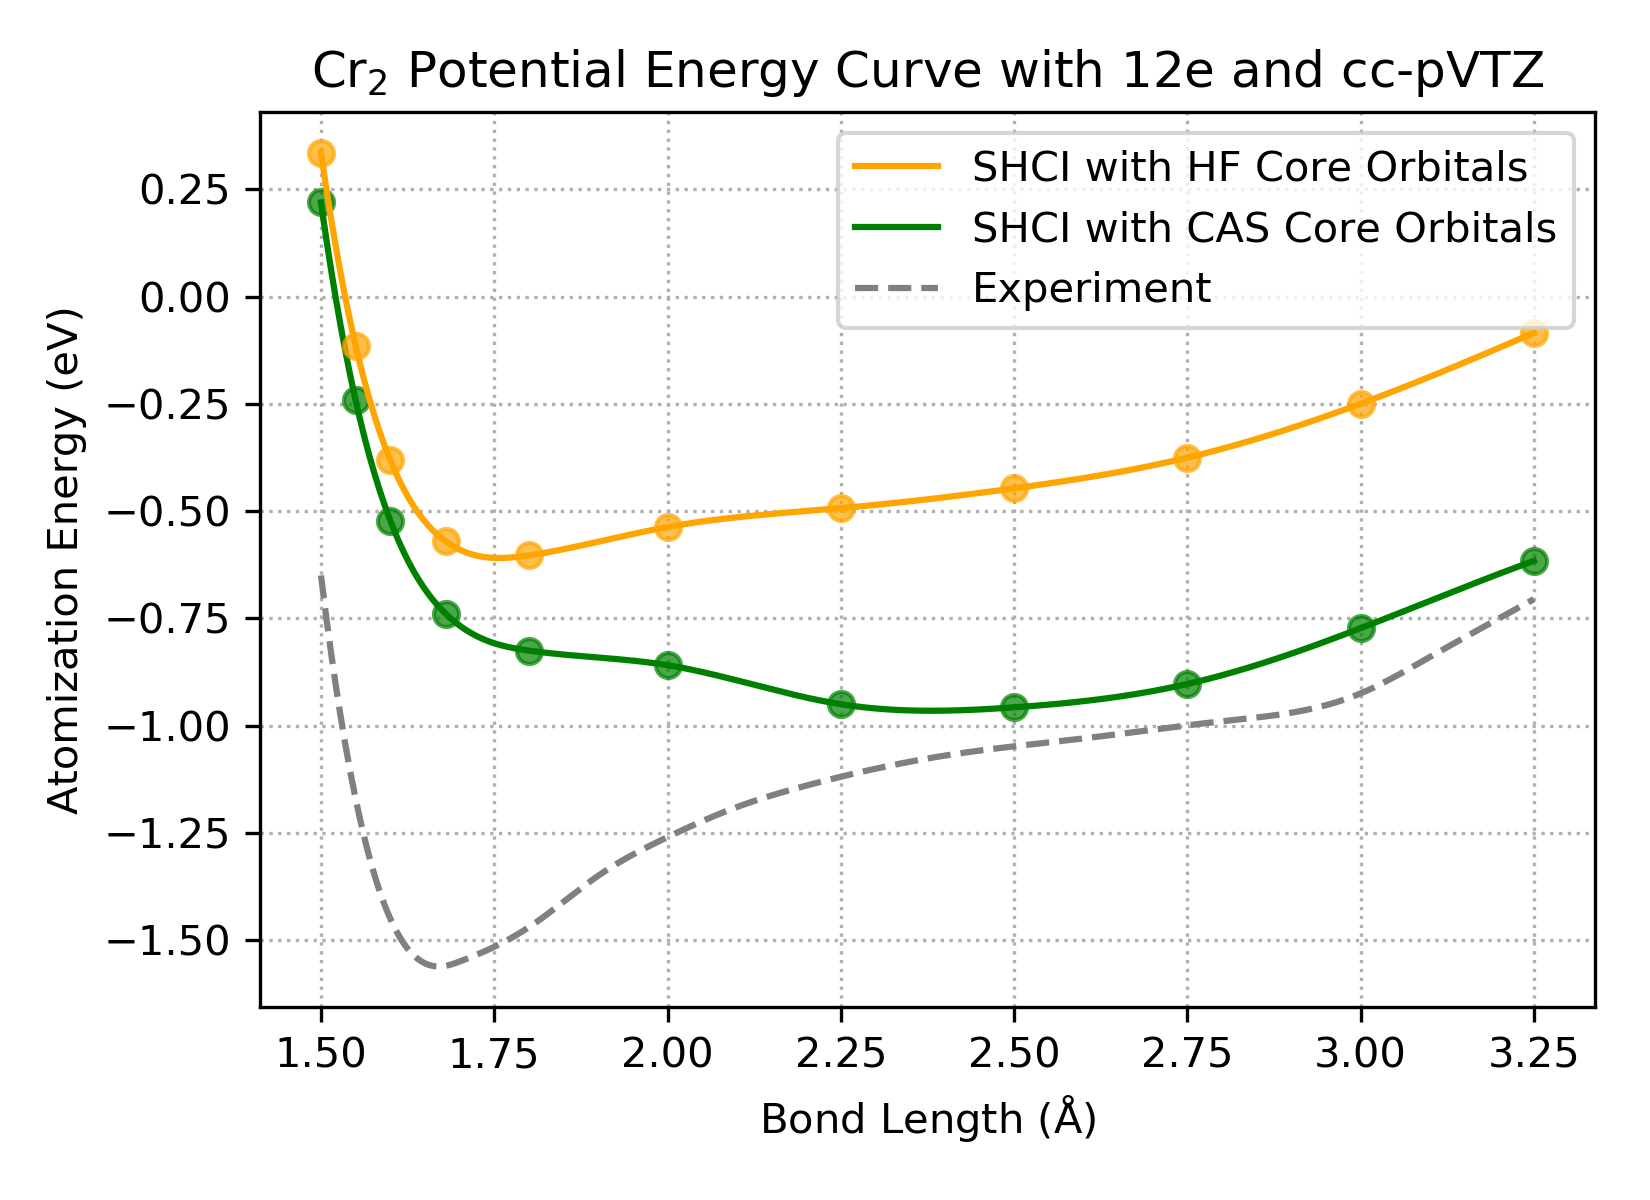
\includegraphics[width=0.9\linewidth]{figs/cashf.png}
  \caption{Comparison of SHCI potential energy curves of Cr$_2$ with 12 correlated electrons and a cc-pVTZ basis, using either HF-core orbitals or CAS-core orbitals.
  The CAS-core curve gives a lower potential energy, closer to experiment, but
  the HF-core calculation results in a potential energy curve whose shape (in particular the location of the minimum)
  is closer to experiment.
  }
  \label{fig:cashf}
  \end{center}
\end{figure}

\begin{figure}
  \begin{center}
  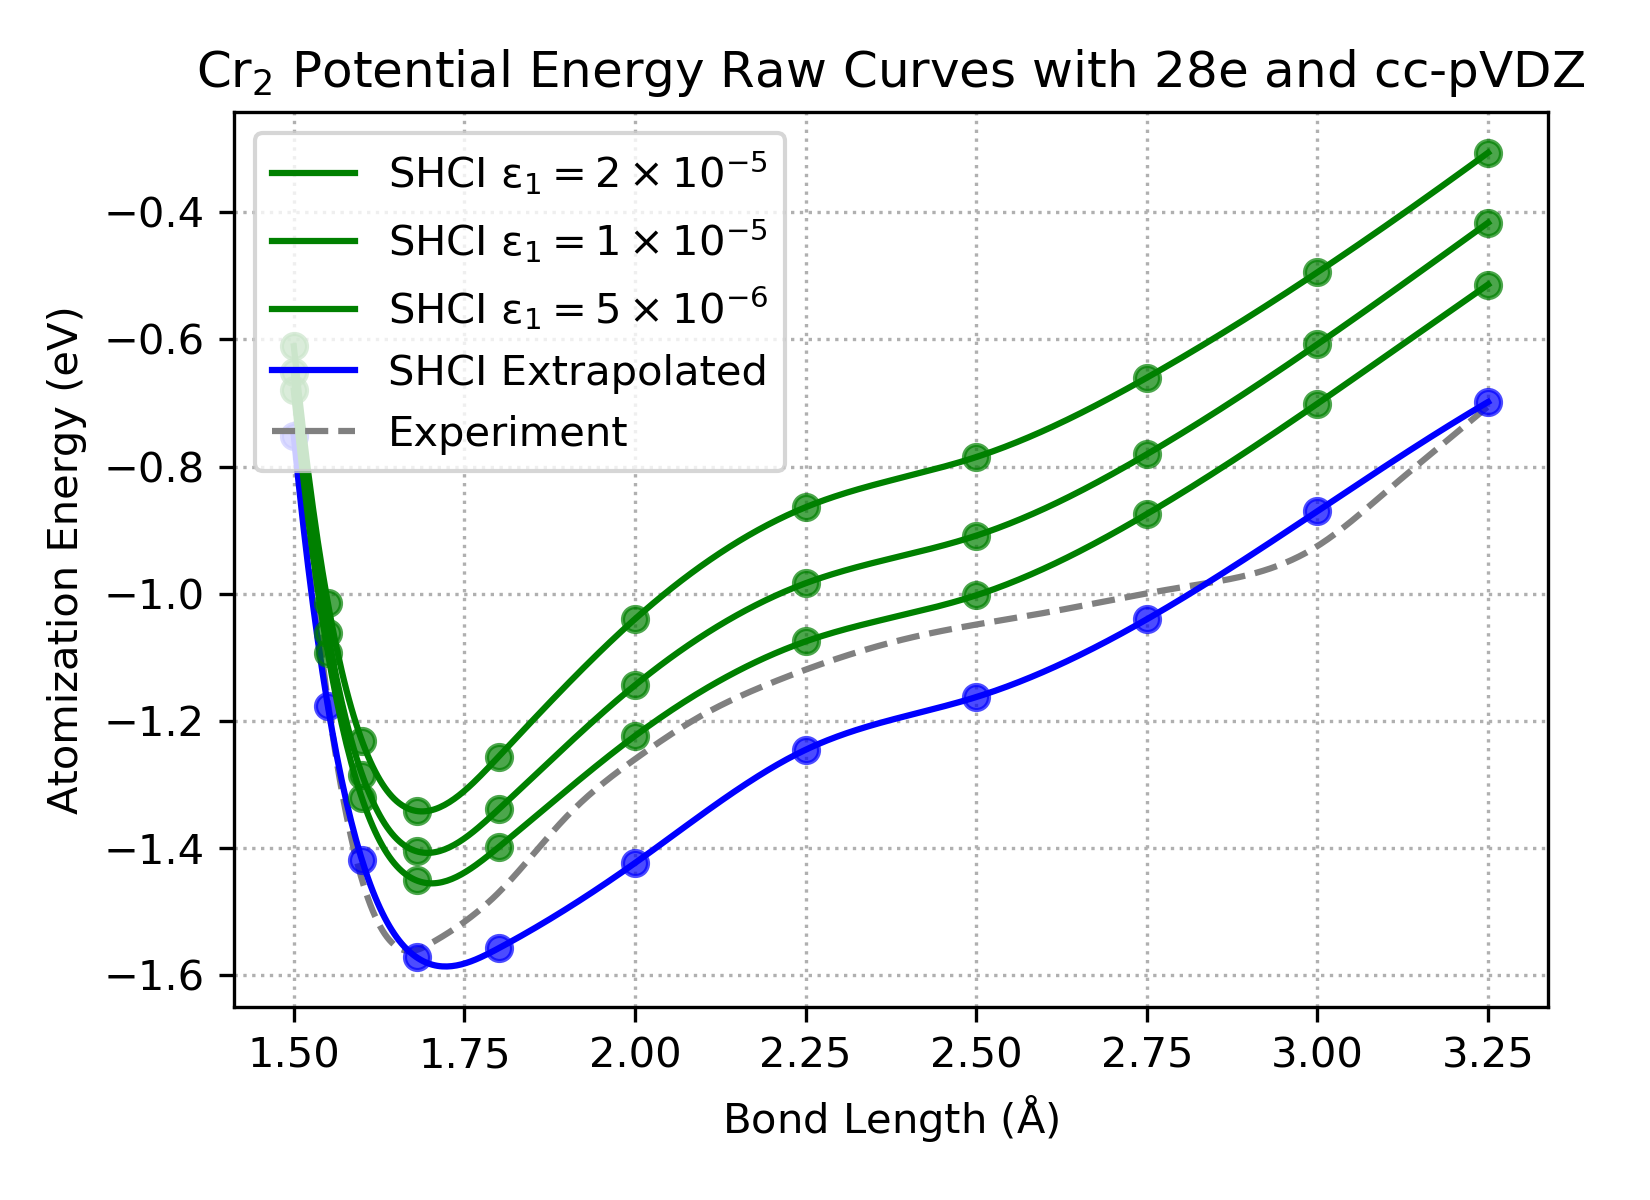
\includegraphics[width=0.9\linewidth]{figs/cr2raw.png}
  \caption{Raw data and extrapolation for Cr$_2$ with 28 correlated electrons and a cc-pVDZ basis.
  }
  \label{fig:cr2raw}
  \end{center}
\end{figure}

\begin{figure}
  \begin{center}
  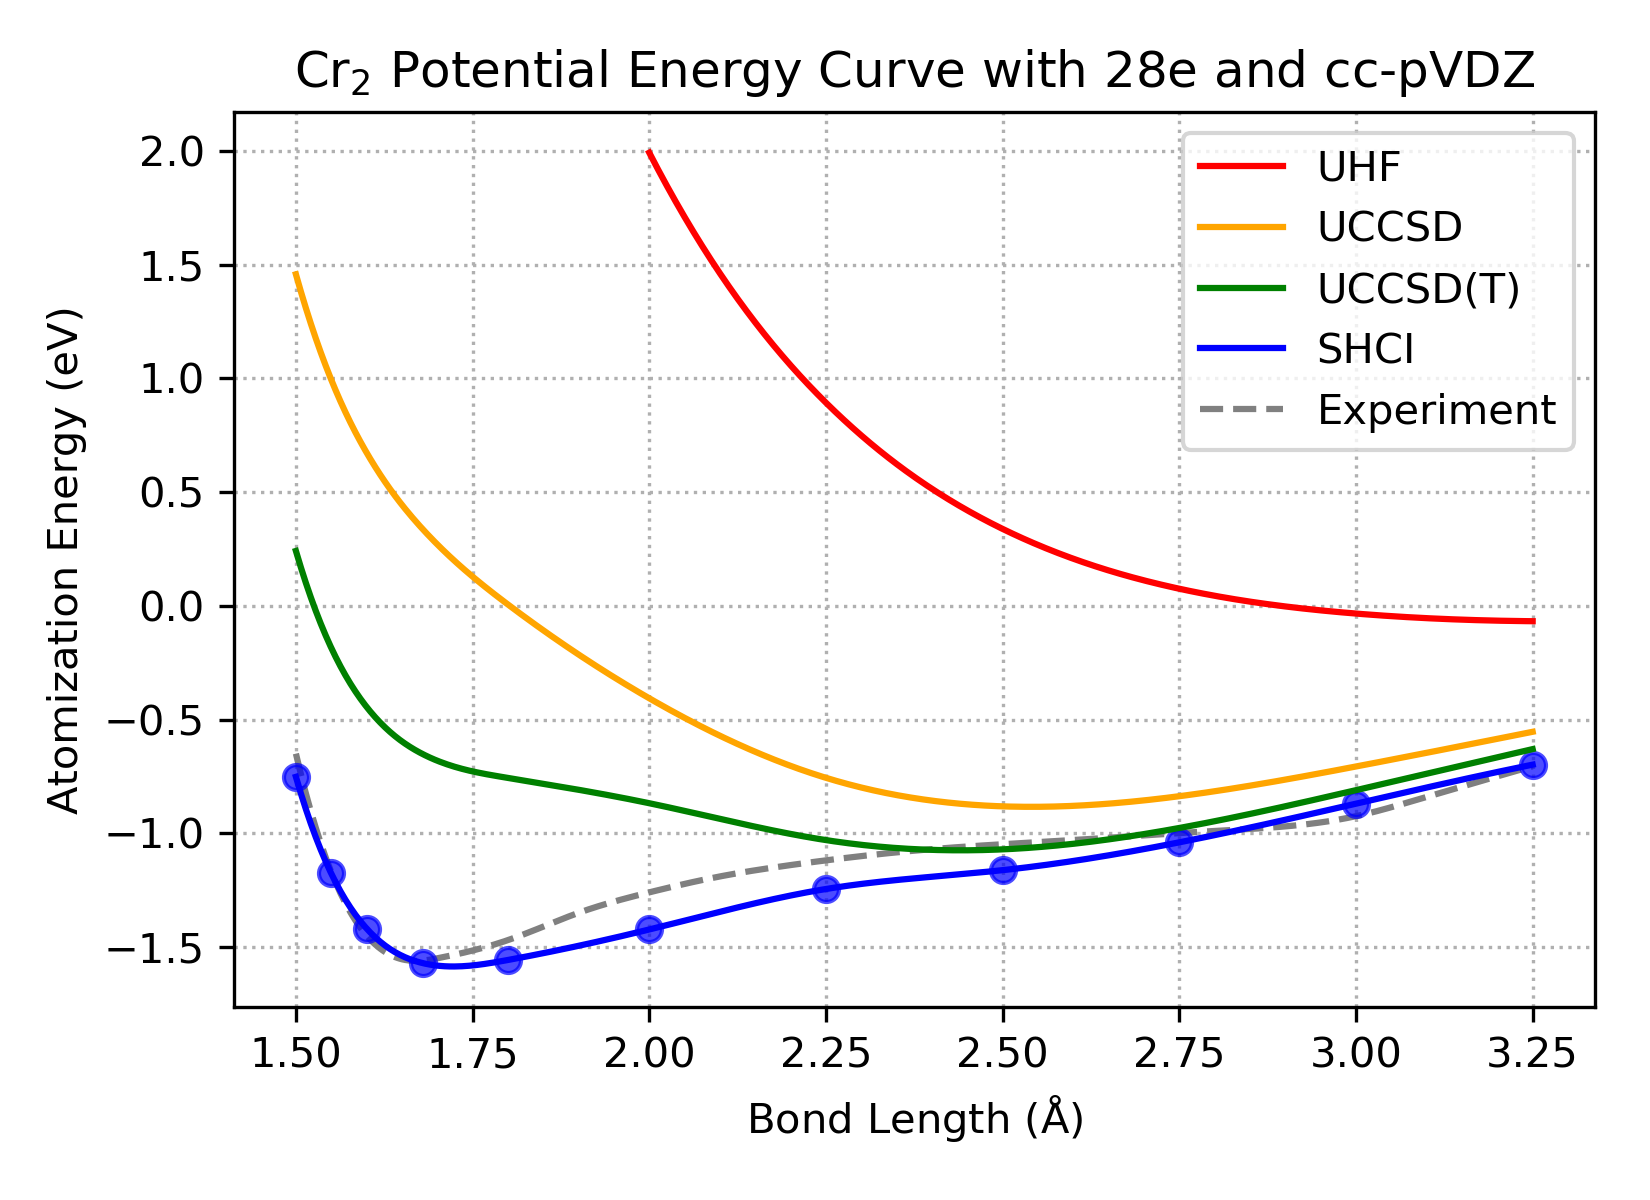
\includegraphics[width=0.9\linewidth]{figs/hfcc.png}
  \caption{Potential energy curve of Cr$_2$ with 28 electrons in a cc-pVDZ basis calculated from various methods.
  The experimental data come from negative-ion photoelectron spectroscopy~\cite{casey1993negative}.
  %We can see that using UHF and CCSD cannot produce a good agreement to the experimental data.
  %CCSD(T) can produce better agreement at stretched geometry but still not good enough near the equilibrium geometry.
  %By using SHCI, the agreement with experimental data is much better.
  The UHF curve bears no resemblance to the experimental curve.
  The UCCSD and UCCSD(T) curves are better, especially at long bond lengths, but even UCCSD(T), which is considered to be the ``gold standard" for single-reference
  systems, agrees poorly with experiment.  In contrast, the SHCI curve is in reasonable agreement with experiment.
}
  \label{fig:hfcc}
  \end{center}
\end{figure}

Fig.~\ref{fig:cr2curve} compares the energies calculated with different active spaces to the experimental data.
There is some uncertainty in the experimental curve due to uncertainty in the assignment of the higher vibrational levels
as well as due to uncertainty in the depth of the potential.
The shape of the experimental curve is deduced from 29 vibrational states using negative-ion photoelectron spectroscopy~\cite{casey1993negative}.
The measured 29 vibrational states were assigned to $\nu=1-9$ and $\nu=24-43$.
There is uncertainty in the shape of the experimental curve because of the missing vibrational levels as well as uncertainty
about the assignment of the observed peaks to the higher vibrational levels.
The depth of the experimental curve is estimated from adding an estimate of the zero-point energy
to experimentally determined bond dissociation energies.
Unfortunately, there is a considerable spread in the estimates of the latter.
Here we use the well depth estimate of 1.56 eV from Ref.~\cite{VanMalVer-JCTC-16}, which is based on the bond dissociation
energy of Ref.~\cite{simard1998photoionization}.
This well depth is deeper than the estimate of 1.47 eV used in Ref.~\cite{GuoWatHuSunCha-JCTC-16} based on
the bond energy of 1.44 eV reported in Ref.~\cite{casey1993negative}.

Fig.~\ref{fig:cr2curve} shows that the 12-active-electron curves do not agree well with experiment.
Using a larger basis sets helps bring the curve closer to the experimental data, but is not enough to produce a good agreement.
By including the 10 additional electrons from the semi-core in the active space, SHCI achieves much better agreement,
demonstrating that semi-core correlation plays an important role in the molecular bond of Cr$_2$.
At large bond lengths one would expect that semi-core correlation is not important and in fact the 12 active electron
and the 28 active electron energies become nearly coincident there.

Fig.~\ref{fig:cashf} shows the difference between using HF-core orbitals and using CAS-core orbital, under the setting of 12 correlated electrons and cc-pVTZ basis sets.
We can see that the CAS-core curve gives a lower potential energy, closer to experiment, but has the wrong minimum location.
The HF-core calculation results in a potential energy curve whose overall shape and the location of the minimum are much closer to the experiment.
                                                                                                                                                                                                                                                                                                                                                                                               
% We can also see from Fig.~\ref{fig:cr2curve} that the effect of using HF core or CAS core for orbital optimization matters little to the 28 electrons SHCI calculation.

%We also compare SHCI results with unrestricted Hartree-Fock (UHF) and low order coupled cluster methods.
In Fig.~\ref{fig:hfcc}, we compare SHCI results to unrestricted Hartree-Fock (UHF) and unrestricted coupled cluster methods, UCCSD and UCCSD(T).
%Fig.~\ref{fig:hfcc} shows the comparison.
%We can see UHF cannot give a good agreement with the experimental data.
%CCSD and CCSD(T) give better agreements for the stretched geometries, but still cannot reach good agreements with the experimental data at compressed or equilibrium geometries.
%SHCI gives good agreement to the experimental data along the entire curve.
As expected, the UHF curve bears no resemblance to the experimental curve.
The UCCSD and UCCSD(T) curves are better, but even UCCSD(T), which is considered to be the ``gold standard" for single-reference
systems, agrees poorly with experiment.  In contrast, the SHCI curve is in reasonable agreement with experiment, perhaps
fortuitously so, since the cc-pVDZ basis used is expected to have a significant finite-basis error.
With our current computer resources, we cannot obtain a well-converged curve with larger basis sets,
but with further improvements in the method and larger computers, we hope to obtain basis set converged curves
that agree yet better with experiment, and perhaps even provide information about experimental inaccuracies.

%Given the resources that we have right now, 28 electrons in a cc-pVDZ basis are the largest configuration that we can do for the entire potential energy curve.
%In the future, as our method keep evolving, and we get more computing resources, we expect SHCI to give even better agreement to the experimental data and can even be used to benchmark the accuracy of experiments on stretches geometries.
